\subsection{System Model}
A high level overview of the ROS2 system used in this study is illustrated in Figure \ref{fig:full_system_diagram}.
The algorithms under test represent the \texttt{AgentLocalizer} box in gold.
It receives sensor data from Gazebo plugins, described below.
Additionally, the \texttt{AgentLocalizer} subscribes to a map representation generated from an octomap\_server node.
The \texttt{AgentLocalizer} publishes its pose to a local motion planner and a position controller.
The position controller then sends commands to a Gazebo DiffDrive \cite{gazebo_diff_drive} plugin which sends joint velocities to the simulated robot's wheels.

\begin{figure}[!htbp]
    \centering
    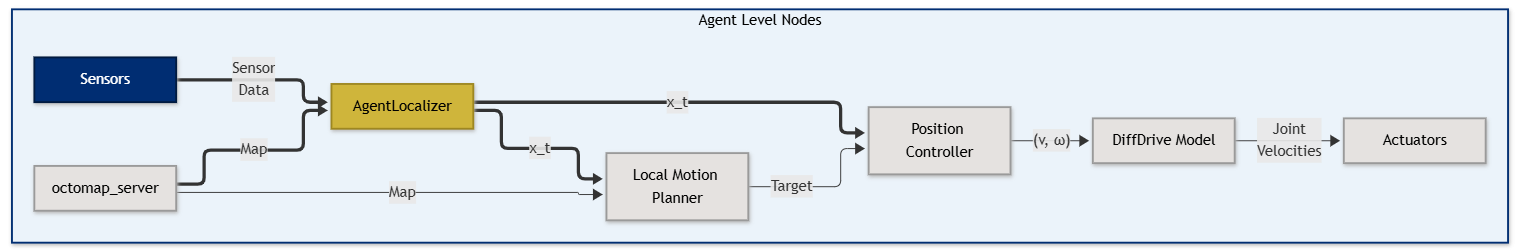
\includegraphics[width=\textwidth]{figures/full_system_diagram.png}
    \caption{Full ROS2 system diagram}
    \label{fig:full_system_diagram}
\end{figure}

The Local Motion Planner and Position Controller nodes are outside of the scope of this work.
In the experiments presented here, the local motion planner uses an RRT* algorithm \cite{karaman2011sampling}.
Both the Local Motion Planner and Position Controller nodes monitor the robot's true position through Gazebo's internal transform tree.
This is done to isolate the localization algorithm's performance without adding complexity.
In a real world application where there is no access to a ground truth transform, these localization algorithms would take the place of the transform tree lookup.

\subsubsection{Platform \& Sensors}
The robot models used in Gazebo and ROS2 are defined using Unified Robot Description Format (URDF).
This study will use the mobile manipulator model illustrated in Figure \ref{fig:devol_robot_model}.
It consists of a Husky A200 differential drive mobile platform with a mounted $270^\circ$ 2-D LiDAR and a manipulator.
The manipulator comprises a Universal Robots UR5e collaborative robot arm and a Robotiq 2F-85 end effector.
Plugins for Differential Drive, odometry, wheel slip, and LiDAR from Gazebo were leveraged to add model the sensors and actuators in the simulated factory.

\begin{figure}[!htbp]
    \centering
    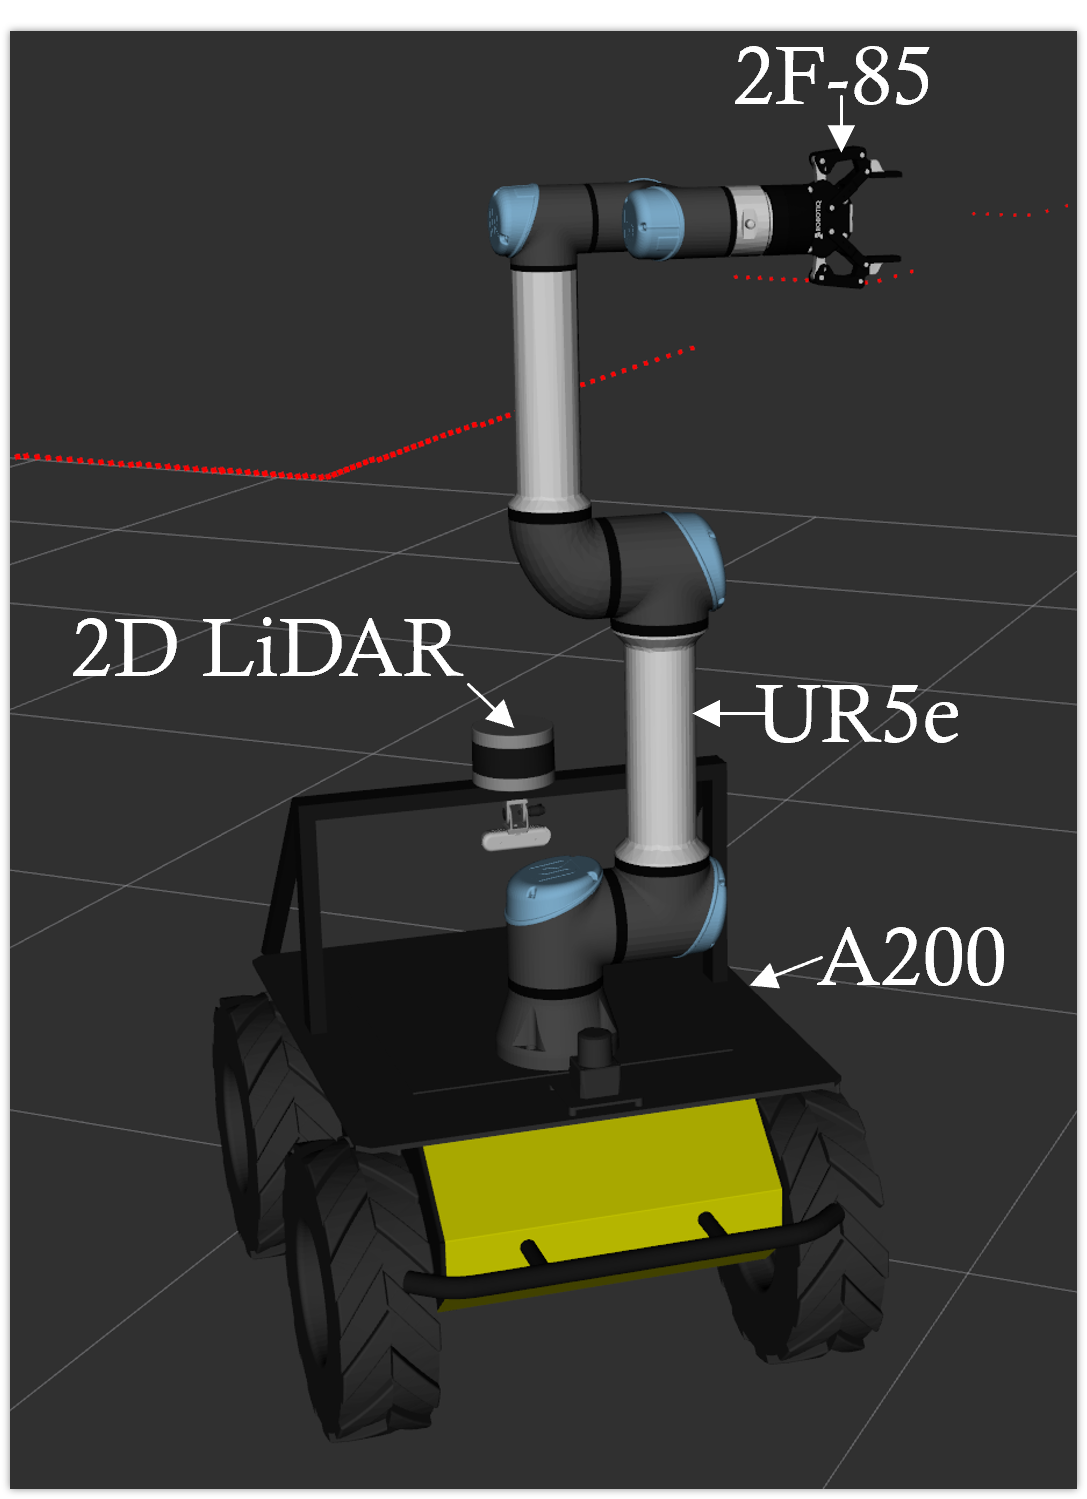
\includegraphics[width=.25\textwidth]{figures/devol_robot_model.png}
    \caption{Test robot model.}
    \label{fig:devol_robot_model}
\end{figure}

\textbf{Odometry:} The \texttt{DiffDrive} plugin \cite{gazebo_diff_drive} is used to both publish \texttt{nav\_msgs/Odometry} messages and receive velocity commands in the form of $u_t=\begin{bmatrix} v_t \\ \omega_t \end{bmatrix}$. 
The \texttt{WheelSlip} \cite{gazebo_wheel_slip} plugin is used to create uncertainty in the odometry to match real world applications.
The robot's odometry publishes at 30 Hz.
Additionally, \texttt{OdometryPublisher} \cite{gazebo_odom} is used to publish the ground truth odometry and transform for results comparison.

\textbf{LiDAR:} The Lidar plugin \cite{gazebo_lidar} is used to generate \texttt{sensor\_msgs/LaserScan} messages.
The beam spans $[\phi_{min},\phi_{max}]=[-2.356,2.356]$.
The transform from the base of the model to the LiDAR frame is static and was calculated with the tf2\_tools as $t_L=[0.32825,0.0,0.0]^T$.
The LiDAR scans are preprocessed by the localization algorithms using the same method.
Rays that are outside of nominal range, as defined by the \texttt{sensor\_msgs/LaserScan} message, are thrown out.

\subsubsection{Unicycle Kinematics}
Since the odometry is produced in the form of $u_t=\begin{bmatrix} v_t \\ \omega_t \end{bmatrix}$, the kinematic model can be reduced to a Unicycle Kinematic model.

\textbf{Forward Kinematics:} The ros2\_controllers page on wheeled kinematics \cite{ros2_control_mobile_robot_kinematics} provides the forward kinematics of the unicycle for continuous time shown in Equation \ref{eq:continuous_unicycle_kinematics}.

\begin{equation}\label{eq:continuous_unicycle_kinematics}
    \begin{bmatrix} \dot{x} \\ \dot{y} \\ \dot{\theta} \end{bmatrix} = \begin{bmatrix}
        v_{b,x}\cos(\theta) \\ v_{b,x}\sin(\theta) \\ \omega_{b,z}
    \end{bmatrix}
\end{equation}

This can be extended to the discrete case as shown in Equation \ref{eq:discrete_unicycle_kinematics}:

\begin{equation}\label{eq:discrete_unicycle_kinematics}
    f(\textbf{x},\textbf{u},\Delta t) = \bar{\textbf{x}}_t = \begin{bmatrix}
        x + v \cos(\theta) \Delta t \\ y + v \sin(\theta) \Delta t \\ \theta + \omega \Delta t
    \end{bmatrix}
\end{equation}

\textbf{State Jacobian:} The state Jacobian $\textbf{A}_t$ is calculated by finding the partial derivatives of equation \ref{eq:discrete_unicycle_kinematics} with respect to $\textbf{x}$.

\begin{equation}\label{eq:state_jacobian_unicycle}
    \textbf{A}_t = \frac{\partial \textbf{f}}{\partial \textbf{x}} = 
    \begin{bmatrix} 
        1 & 0 & -v \sin(\theta) \Delta t \\
        0 & 1 &  v \cos(\theta) \Delta t \\
        0 & 0 & 1
    \end{bmatrix}
\end{equation}

\textbf{Control Jacobian:} The control Jacobian $\textbf{G}_t$ is calculated by finding the partial derivatives of equation \ref{eq:discrete_unicycle_kinematics} with respect to $\textbf{u}$.

\begin{equation}\label{eq:control_jacobian_unicycle}
    \textbf{G}_t = \frac{\partial \textbf{f}}{\partial \textbf{u}} = 
    \begin{bmatrix} 
        \cos(\theta) \Delta t & 0  \\
        \sin(\theta) \Delta t & 0  \\
        0 & \Delta t
    \end{bmatrix}
\end{equation}

\subsubsection{Odometry Noise Model}
Chapter 5 of \textit{Probabilistic Robotics} by Thurn \cite{thrun2005probabilistic} provides algorithms for injecting noise into our odometry sensors.
The book argues that command states or measured sensor are subject to noise and that noise can be modeled by a zero-centered random variable with finite variance as Equation \ref{eq:motion-noise}.

\begin{equation}\label{eq:motion-noise}
    \binom{\hat{v}}{\hat{\omega}} = \binom{v}{\omega} + \binom{\sigma_{\alpha_1 \left\lvert v \right\rvert + \alpha_2 \left\lvert \omega \right\rvert}}{\sigma_{\alpha_3 \left\lvert v \right\rvert + \alpha_4 \left\lvert \omega \right\rvert}}
\end{equation}

All three algorithms in this study, leverage this concept to model the uncertainty of the odometry.
Where $\alpha_1=0.10$ represents the translational noise caused by translation.
$\alpha_2=0.01$ represents the translational noise caused by rotation.
$\alpha_3=0.01$ represents the rotational noise caused by translation.
And $\alpha_4=0.20$ represents the rotational noise caused by rotation.
These values are used to create noise proportional to the odometry control signal $u_t$ as shown in Equations \ref{eq:v-noise} and \ref{eq:omega-noise}.

\begin{equation}\label{eq:v-noise}
\sigma_v = \alpha_1 |v_t| + \alpha_2 |\omega_t|
\end{equation}
\begin{equation}\label{eq:omega-noise}
\sigma_\omega = \alpha_3 |v_t| + \alpha_4 |\omega_t|
\end{equation}

\subsubsection{Map}
The open source \texttt{octomap\_server} \cite{hornung2013octomap} is used to generate the static map.
A Point Cloud Data (PCD) file was generated of the gazebo world using the open-source \texttt{sdf2map} package \cite{sdf2map}.
The static PCD file is provided to the \texttt{octomap\_server} at runtime which then publishes an OctoGrid with $0.05m$ resolution and an OccupancyGrid which is a 2-D projection of the OctoGrid.
The bottom $0.45m$ of the point cloud is removed before applying the projection to keep the factory floor from occluding the free space.
